



What are the public health, safety and welfare, global, cultural, societal, environmental, 
and economic factors related to the problem and solution space? What power does the proposed system 
provide, and to whom? What are the relevant professional ethical obligations to consider in the design 
of the system?

\subsection{Factors Related to the Problem and Solution}

\subsubsection{Public Health, Safety, and Welfare}
The main issue the proposed system addresses is the potential for negligent discharge of a firearm. This is because of the nature of guns in that the are designed
to inflict harm on a target. The smart trigger would help to protect the public safety in a couple of ways. First the system would be designed to prevent the gun from 
firing unless it is used by the owner. This would help to prevent accidental shootings by children or others that are not lisenced to shoot a firearm. Secondly, if the gun was lost unless
the module was removed the gun wouldn't be able to fire. This would help to prevent the gun from being used in crime or from being used in a negligent way. 
Lastly, the system is module meaning that if at any point it has a malfunction the module can be removed and the gun can be used as normal. 
This would help to prevent situtation where a gun is rendered unusable due to malfucntions of the system. In the past since the mid 1990s, there have been numerous 
starts to create something similar to the smart trigger. These safety devices are known as Firearm Safety Devices (FSDs) and are most of the time mechanical as 
they are reliable and don't require a power source as shown in fig \ref{MechFSD}.

They also have some characteristics and features that are mentioned in \cite{devices2013personalized} 
\begin{itemize}
    \item the option of integrating and combining mechanical devices with various authorization processes (token, password, biometric);
    \item hierarchical authorization;
    \item traceability and logging functions;
    \item networking and remote availability.
\end{itemize}


\begin{figure}[H]
    \centering
    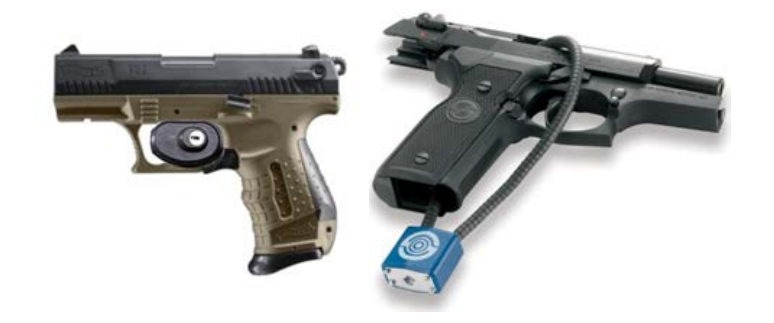
\includegraphics[width=0.5\textwidth]{../Figures/Mech_FSD.png}
    \caption{Trigger and Cable Lock}
    \label{MechFSD}
\end{figure}

\subsubsection{Global, and Cultural}

Because our project is focused on firearms it is impotant to consider the global and cultural factors that may affect the implementation and use of the smart trigger. 
For example, different countries have different laws and regulations regarding firearms, and the cultural attitudes towards guns can vary significantly. 
It is important to ensure that the system is designed in a way that is compliant with these regulations and respectful of these cultural differences. For the scope of the
project we will be focusing on the United States, but it is also important to consider its implications in other countries.
The United States has a deep history with firearms and the Second Amendment to the Constitution guarantees the right of citizens to keep and bear arms. This doesn't mean 
that no regulations have been put in place regarding firearms. Some laws that may affect the system include:
\begin{itemize}
    \item Maryland (SB 334/HB 1339) This law requires that all firearms be equipped with a safety device before being sold or transferred. In order for our system to
    approved in Maryland it would need to be approved by the Handgun Roster Board, which is responsible for evaluating and approving firearms and firearm safety devices for sale in the state.
    \item New Jersey's "Display Mandate": This law requires that all firearms be displayed in a visible manner when being sold or transferred. This would require the entire
    state to adopt the smart trigger as the standard to use in New Jersey.
    \item Because our system uses RFID technology its legaly and intential radiator. This means that if we ever wanted to sell the system in the United States we would 
     need to get approval from the Federal Communications Commission (FCC) to ensure that it complies with regulations regarding radio frequency emissions.
\end{itemize}
 
\subsubsection{Societal and Economic}

Part of the reason why the RFID authentication would be benefictial is that it would be a more affordable and reliable solution compared to other biometric authentication methods. 
This would make it more accessible to a wider range of gun owners, which could help to increase the adoption of the system and ultimately improve public safety. At gun ranges unless
the user was wearing the RFID tag they wouldn't be able to use the gun. This would make shooting ranges safer for everyone because it would prevent unauthorized users from using the guns.
This would also help to prevent accidents and injuries at shooting ranges, which could have a positive impact on public health and safety. Another way in which the system
would increase safety is if a gun was lost or stolen from the police department. If the gun was equipped with the smart trigger it would be rendered useless to any thief.

For each of the 

% Please add the following required packages to your document preamble:
% \usepackage[table,xcdraw]{xcolor}
% Beamer presentation requires \usepackage{colortbl} instead of \usepackage[table,xcdraw]{xcolor}
\begin{table}[H]
\begin{tabular}{l|l|}
{\color[HTML]{595959} Microcontroller}                       & {\color[HTML]{595959} \$15 or free}                            \\
{\color[HTML]{595959} RFID Scanner}                          & {\color[HTML]{595959} $9 prototype board, $3-5 per chip}       \\
{\color[HTML]{595959} AR-15 Lower}                           & {\color[HTML]{595959} Free (thanks Stephen)}                   \\
{\color[HTML]{595959} 3D Printed Parts}                      & {\color[HTML]{595959} \$20 maximum}                            \\
{\color[HTML]{595959} Custom PCB}                            & {\color[HTML]{595959} \$50 in prototyping, $\sim$25 per order} \\
{\color[HTML]{595959} Various electronic parts for the PCBs} & {\color[HTML]{595959} \$20-50}                                 \\
{\color[HTML]{595959} Linear Actuator}                       & {\color[HTML]{595959} \$20}                                    \\
{\color[HTML]{595959} RFID Tags}                             & {\color[HTML]{595959} $10 for prototypes, $10 for the ring}    \\
{\color[HTML]{595959} RFID Programmer}                       & {\color[HTML]{595959} \$30}                                    \\
{\color[HTML]{595959} Battery}                               & {\color[HTML]{595959} $10 for battery, $5 for charger parts}   \\
{\color[HTML]{595959} \textbf{Total}}                        & {\color[HTML]{595959} \textbf{\$190-235}}                     
\end{tabular}
\end{table}

\subsubsection{Environmental}

    The use of RFID technology in our system also has some environmental considerations. 
    The production and disposal of the RFID tags and other electronic components can have an impact on the environment. 
    However, we will strive to use sustainable materials and practices wherever possible to minimize this impact.


\subsection{Power}

Understanding how the system could be used and how power is shifting is important to ensure that the system is designed in a way that is ethical and responsible.
The smart trigger would provide power to the gun owner by allowing them to have more control over who can use their firearm. This would help to prevent unauthorized use of the gun, 
which could improve public safety and reduce the risk of accidents and injuries. This would also give power to law enforment by making it more difficult for stolen
guns to be used in crimes and against police officers in shoot outs. The system would also provide power to the general public by helping to prevent accidents and injuries caused by negligent discharge of firearms.
If the system were to have any bugs or issues it could potentially be exploited by moving power to the criminals. 



